


\subsubsection{UCA 7 - Autenticazione con credenziali LDAP}%kite level

\begin{figure}[h]
	\centering
	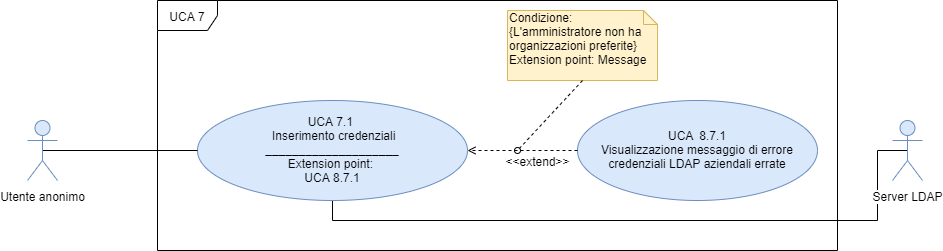
\includegraphics[scale=0.4, center]{sezioni/UseCase/Immagini/UCA7.png}
	\caption{UCA 7 - Autenticazione\ap{G} con credenziali LDAP}
\end{figure}

\begin{itemize}
	\item \textbf{Attori primari:} Utente anonimo 
	\item \textbf{Attori secondari:} Server LDAP\ap{G} dell'organizzazione\ap{G}.
	\item \textbf{Precondizione:} L'utente è autenticato con le proprie credenziali Stalker.
	\item \textbf{Postcondizione:} L'utente è autenticato all'interno dell'organizzazione\ap{G} con credenziali LDAP\ap{G}.
	\item \textbf{Scenario principale:} L'utente autenticato come utente anonimo effettua l'autenticazione\ap{G} con credenziali LDAP\ap{G} [UCA 7.1] per autenticarsi come utente riconosciuto all'interno della relativa organizzazione\ap{G}.
\end{itemize}

\subsubsection{UCA 7.1 - Inserimento credenziali}
\begin{figure}[h]
	\centering
	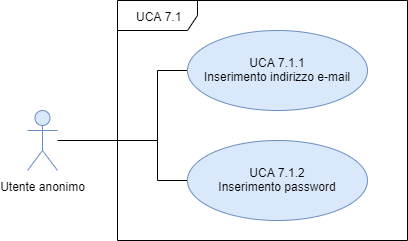
\includegraphics[scale=0.5, center]{sezioni/UseCase/Immagini/UCA7.1.png}
	\caption{UCA 7.1 - Inserimento credenziali}
\end{figure}

\begin{itemize}
	\item \textbf{Attori primari:} Utente anonimo 
	\item \textbf{Attori secondari:} Server LDAP\ap{G} dell'organizzazione\ap{G}.
	\item \textbf{Precondizione:} L'utente  autenticato con le proprie credenziali Stalker.
	\item \textbf{Postcondizione:} L'utente ha inserito le proprie credenziali LDAP\ap{G}.
	\item \textbf{Scenario principale:}: L'utente inserisce le proprie credenziali LDAP\ap{G} per potersi autenticare.
	\item \textbf{Flusso di eventi:}
	\begin{enumerate}
		\item L'utente inserisce il proprio nome utente [UCA 7.1.1];
		\item L'utente inserisce la password [UCA 7.1.2].
	\end{enumerate}
	\item \textbf{Scenario alternativo:} Il tentativo di autenticazione\ap{G} fallisce perché le credenziali inserite sono errate [UCA 8.7.1].
	\item \textbf{Estensioni:}
	\begin{itemize}
		\item UCA 8.7.1 - Visualizzazione messaggio di errore credenziali LDAP aziendali errate.
	\end{itemize}
\end{itemize}

\subsubsection{UCA 7.1.1 - Inserimento nome utente}%fish level
\begin{itemize}
	\item \textbf{Attori primari:} Utente anonimo
	\item \textbf{Precondizione:} L'utente deve inserire il proprio nome utente.
	\item \textbf{Postcondizione:} L'utente ha inserito il proprio nome utente.
\end{itemize}

\subsubsection{UCA 7.1.2 - Inserimento password}%fish level
\begin{itemize}
	\item \textbf{Attori primari:} Utente anonimo
	\item \textbf{Precondizione:} L'utente deve inserire la propria password
	\item \textbf{Postcondizione:} L'utente ha inserito la propria password.
\end{itemize}
